\documentclass[12pt]{article}
\usepackage{multicol}
\usepackage{caption}
\usepackage[a4paper, total={7in, 10in}]{geometry}
\usepackage{titling}
\usepackage{titlesec}
\usepackage{graphicx}

\graphicspath{{/home/cmilanese/Desktop/school/machine_learning/git_repo/docs/images/}}

\title{\Huge \textbf{Techniques comparison for music generation}}
\author{
      \small Milanese, Cristiano \\ \small 2600169
      \and
      \small Hopkinson, Joe \\ \small 2612836
      \and
      \small Bertozzini, Gregorio \\ \small 2619064
      \and
      \small Herbeaux, Etienne \\ \small 2608599
      \and
      \small Hotanu, Razvan \\ \small 2623943
}
\date{}

\titleformat{\section}
  {\normalfont\huge\bfseries}{\thesection}{1em}{}[{\titlerule[0.8pt]\vspace{0.3cm}}]
\titleformat{\subsection}
  {\normalfont\fontsize{14}{18}\bfseries}{\thesection}{1em}{}

\begin{document}
\maketitle
\begin{center}
\textbf{How effective is an LSTM for music generation when compared to \\ probabilistic music generation using the markov model?}
\end{center}
\vspace{10pt}
\section*{Abstract}
  Introducing machine learning models, the first decision we are called to make is whether the scope of our research focuses on classification or generation. This two concepts tightly relate to their learning process. A discriminative model maps directly into classification problems, shaping the decision boundary between the inputs in order to infer the class of a particular instance, while the generative one takes into consideration the joint probability distribution, namely the likelihood of an input instance to belong to a class rather than another.
\section*{Introduction}
   Musical composition is an inherently creative and human exercise. Despite modern western music following some degree of mathematical structure, there remains a significant aspect of subjectivity to its construction and evaluation. As such there remains the question of whether machine learning can be used to generate a piece of music that is potentially indistinguishable from manually written works. In this research paper, we aim to investigate how both probabilistic and deep learning techniques can be used to generate a musical composition given a library of classical music to learn from.
\section*{Data inspection and preparation}
\subsection*{MIDI format}
  \begin{flushright}
    \begin{minipage}[t]{0.96\linewidth}
      MIDI is a universal format of encoding musical sequences that, unlike a traditional WAV or MP3 formats, can be manipulated and edited on a note-to-note basis and offers a high level of detail regarding the sequencing of the music [9]. The hexadecimal file is structured as a series of chunks: a header file consisting of metadata relating to global properties of the file followed by numerous track chunks that contain sequence specific data. This metadata allows access to the theoretical properties of the song such as key signature, time signature, number of tracks format, and other file specific information. For the purpose of this research, we are only concerned with the 'note on' / 'note off' MIDI events as they give us the data regarding which note is being played at a given time stamp. From this it is possible to arrange the sequential sequence of notes that a song follows.
    \end{minipage}
  \end{flushright}
\subsection*{Theoretical music concepts}
  \begin{flushright}
    \begin{minipage}[t]{0.96\linewidth}
      In order to generate a cohesive musical sequence, and later evaluate its quality, it is necessary to outline the theoretical properties of compositions that make them musical [5], as opposed to a random sequence of notes. It is important to state that although there is a significant mathematical aspect of musical composition, there is likewise some degree of subjectivity to both the construction and the evaluation of its quality [6]. This presents a challenge for a machine learning model to distinguish a 'good' sequence from 'bad' one.  As such it is important to establish the methodology and metrics that can be used to attempt to quantify a musical sequence of notes. \\ The musical alphabet consists of 12 notes ranging from A to G, with a number of flats/sharps interspersed. Imagining a piano, the keys represent the notes over a number of octaves (or pitches) with different intervals between the notes. For example the interval between C and C\# (Db) would be a half step, also known as a semitone. These intervals form the foundation of melody in music. Musical compositions can be written in either major or minor, and this relates to the scale that the notes in the song belong to. The difference between the scales relate to the intervals between the notes.
      \vspace{10pt}
      \noindent\makebox[\textwidth][c]{%
        \begin{minipage}{0.4\textwidth}
          \vspace{10pt}
          Major: 2 - 2 - 1 - 2 - 2 - 2 - 1 \\*
          Minor: 2 - 1 - 2 - 2 - 1 - 2 - 2
        \end{minipage}}
      The key signature of a song entails the type of scale a song uses, along with the scales starting note. For example a song in C major would use the following notes:
      \vspace{10pt}
      \noindent\makebox[\textwidth][c]{%
        \begin{minipage}{0.4\textwidth}
          \vspace{10pt}
            C D E F G A B C
        \end{minipage}}
      The key signature of a song entails the type of scale a song uses, along with the scales starting note. For example a song in C major would use the following notes: C D E F G A B C. This is because these are the notes that follow the intervals of the major scale, starting with the note A. Although some genres of music are more flexible regarding their compliance with this rule, it is possible to assume that most western music does follow this principle to a high degree. Having access to the musical sequence along with its key signature allows us to quantify to some degree how melodic the generated musical sequence is.
    \end{minipage}
  \end{flushright}
\subsection*{Data exploration}
  \begin{flushright}
    \begin{minipage}[t]{0.96\linewidth}

    The initial dataset that was obtained for this project consisted of a library of approximately 300 classical MIDI files acquired from the University of Minnesota's School of Music e-competition online library. A web script was run on the site to condense the various files into one directory for our models to access. Upon exploring these MIDI files, it soon became apparent that despite the MIDI format accommodating key signature meta events enclosing such information, the reality is that a high percentage of files lacked this data. This presented a significant problem for our research. As discussed above, it is not necessarily the notes themselves that contribute to a melodic sequence, rather the intervals between them and the patterns they form. For example the notes C, D have the same relationship as A, B as they are the first two notes in the C major scale and the A major scale. Without the key signature however, it is not possible to determine this relationship, and therefore our models will be unable to distinguish what follows a pattern and what doesn't. The initial intention was to normalise all the files in our dataset to one particular key in order to compare the relationships between notes for all songs, however this is not possible to do without the key data. \\*

    Upon research [8], it was determined that it is possible to implement an algorithm that can approximate the key of a song in various ways. One naive method does so by comparing a song's notes to the 12 diatonic major scales, with an additional weighting multiplier for the key root note. Although this supposedly can be done to a reasonable degree of accuracy, 100\% accuracy can never be achieved due to the possible subjectivity of this property.  This uncertainty posed as a possible bottleneck for our final generated sequences. Because of this, it was determined that a more reasonable solution to the absent key problem was to manually obtain files from multiple resources [10][11] to each corresponding key. This method allows us to know with absolute certainty what key each particular song is in so that it can be normalised as input for the models. The final generated output will then be representative of the performance of the model rather than the performance of a key estimator. \\*

    Another important decision that was taken was to focus solely on songs written in the major scales as opposed to minor. As demonstrated above, major and minor scales have different interval patterns and therefore would have to be separated when it comes to running the models. It was concluded that the minor addition would not enhance the results and would simply overcomplicate both the dataset and the learning process. The final dataset consisted of approximately 300 files from 4 major keys: C, E, F, G, normalised to C. \\*
    As a baseline for our generated sequences to be referenced against, this dataset was inputted to the function that calculates the percentage of notes in the song that exist in the scale of the songs key. The average percentage was 80.5\%. This confirms that although the majority of the songs do follow the basic musical principles discussed above, due to variations in genres and song writing approaches, not all do thus confirming the difficulty of mathematically evaluating melodies.
    \end{minipage}
  \end{flushright}
\section*{Methodologies}
\subsection*{Hidden Markov Model}
  \begin{flushright}
    \begin{minipage}[t]{0.96\linewidth}
       In order to represent the sequential nature of our input we first decided to apply an intuitive solution, namely a probabilistic model, the hidden Markov Model. Markov Model has been successfully applied to a wide range of sequence analysis problems and it used to be the standard for audio/music generative models because the process behind the Markov Models are very suitable for music composition[7, p.11]. However, the Markov model has slowly faded away because of its lack of memory, being an instance-based model that does not learn like other machine learning models. In fact, it does not learn directly from the data, but rather the data is the source from which we can produce our probabilistic table[7, p.11]. We created a table indicating the probability of each note in comparison with the previous one, and through this table we predicted the second generated note, the first being randomly generated. Now we should not focus on finding the most probable note linked with the lastly generated note, but with a sequence of two notes instead, referenced as Y. Markov models are a first approach we can take on this sort of data through the creation of the Markov assumption, which implies a limited memory. Using this, we can pretend that the current note depends on the previous two notes, so our model becomes a 2nd order Markov model. From now on we want to know what is the probability of having this sequence X from the learned one. The sequence X is defined as the bigram, Y, previously generated plus a randomly sampled note, defined as G. Then we need to evaluate this X sequence in a probabilistic way, calculating the conditional probability of G given the bigram Y. In order to determine this conditional probability we want to count the occurences of sequence X and divide them by the occurrences of the bigram Y. We want to try as many different G as possible, where the probability of X is bigger than zero, so we will have a very broad probabilistic range. From here we choose between the best three trigram options, having the highest probability; 50\% from the most probable, 30\% the second most probable, 20\% the third most probable. After choosing the trigram the new note is added to the generated notes. This randomness will make sure that our generated song will not get stuck into loops of fews notes and it will give a bit of randomness and creativity to the newly generated songs.
    \end{minipage}
  \end{flushright}
\subsection*{from Machine Learning to Generative models}
  \begin{flushright}
    \begin{minipage}[t]{0.96\linewidth}\
      Moving on from multilayer perceptron and classical machine learning methods, CNNs adopt convolutional operation at their hidden layer phases to detect patterns from the input data. The main difference with a fully connected layer is that we are able to retain the spatial factor or shape of our input. This operation is achieved by defining what, in image processing jergon, is called a kernel or filter. Taking the dot product of the input with this filter results in new mappings, each defining an important characteristic of the input. Lastly, a fully connected layer would be hooked to our model in order to produce a score function and rank our guessed outputs. What prevented us from using CNN for our project, despite keen to preserve the initial shape of the data, is the lacking ability to deal with sequential data, one of the prevalent features of songs, read as sequences of notes.
    \end{minipage}
  \end{flushright}
\subsection*{Recurrent Neural Net}
\begin{flushright}
  \begin{minipage}[t]{0.96\linewidth}\
    Our focus, therefore, moved towards specialized models for sequence analysis, such as Recurrent Neural Nets. These architectures are good at modelling sequences of data, among its applications we  often encounter natural sequences analysis such as for audio or text. Common to other machine learning models, RNNs share a structure of input, hidden and output layers connected via weighted functions, but they are equipped with loops at the hidden layers in order to render the information persistent. They use hidden states as memory cells, passing on each of their outputs to the following cell, which vector is then concatenated with the following input, collecting information coming from previous states. As with other models, after each forward pass, the neural network performs backpropagation in order to learn, but under this shape our model is not able to retain previous iteration and we would end up learning only from the last. Backpropagation through Time is a technique applicable to unrolled models, namely the version of what we have built so far with all temporal passes withheld in memory. Yet this version suffers from the vanishing gradient problem, embedded in the nature of backpropagation as the update method for the various weights of the hidden layers. Its value shrinks until it is so small that it does not contribute to learning anymore, as opposed to the cases in which it grows far off the learning boundary. The main consequence of this issue is that vanilla RNN struggles to remember long sequences of input.
  \end{minipage}
\end{flushright}

\subsection*{Long-Short Term Memory architecture}
\begin{flushright}
  \begin{minipage}[t]{0.96\linewidth}\
    Finally, inspired by previous work on music generation, we applied a specialized form of vanilla RNN that solves the issue of vanishing gradient descent, allowing the net to remember longer sequences by forgetting some information along the way. This all process is implemented through gates, which filter out parts of the sequences that are not relevant. Three different gates are responsible for regulating information in a cell:
    \begin{itemize}
      \item \textbf{input gate} collects data from the current input and compares it with the previous one, applying a sigmoid activation function
      \item \textbf{forget gate} decides which information is to be kept, the sum of the previous (hidden) state and the current state are passed onto a sigmoid activation function.
      \item \textbf{output gate} provides the output data for the following layer of the network, multiplying current cell state with the input and normalizing it through both tanh and sigmoid activation functions.
    \end{itemize}
  \end{minipage}
\end{flushright}
\subsection*{Training}
\begin{flushright}
  \begin{minipage}[t]{0.96\linewidth}\
    Our input data is defined as a univariate distribution, as each of the notes has a single feature, being the midi value they are represented in. Inspired by [1] we created a model that includes 3 LSTM layers each composed of 512 nodes, followed by a batch normalization layer, a technique first introduce by Sergey Ioffe in his 2015 paper [2] in order to adjust and scale the activation functions, stabilize the network and avoid internal covariance shifts. A subsequent dropout layer, as established by Srivastava et al. [3], ensures that the least important nodes in the model get discarded and do not affect the output by overfitting the data. Lastly, a dense layer reduces the dimensionality of the output to conform to the number of possible outputs and apply a softmax activation function, so we can read the outcome as probability distribution and their values sum up to 1. The model is compiled using categorical cross-entropy loss as a forced choice given that we want to backpropagate the loss over categorical data (although imported as their pitch number rather than their names), in addition we use rmsprop optimizer to speed up the convergence of the loss function, which is a technique very similar to gradient descent with momentum.
  \end{minipage}
\end{flushright}
\subsection*{Label forecasting}
\begin{flushright}
  \begin{minipage}[t]{0.96\linewidth}\
    The output values are one-hot encoded so that the model is able to predict a class for each current input sequence. The prediction is then appended to the current sequence in order to foresee the following note. This method is called Sequence to Label generation.
  \end{minipage}
\end{flushright}
\subsection*{Technical information}
\begin{flushright}
  \begin{minipage}[t]{0.96\linewidth}\
    In order to implement this, we are using TensorFlow’s Keras API for deep learning. Categorical cross-entropy is used as a loss function for single label categorization, which compares the distribution of the predictions with the true distribution. For the optimizer we use RMSprop which uses the adaptive learning rate.
    In order to speed up the process of training the model, we made use of TensorFlow’s GPU integration which relies on cuda support for dedicated graphics cards, paired with a Nvidia Geforce GTX1060. This led to varying weights and loss values across the training period of the model. The initial loss started at around 5 with big changes in the beginning as expected. As the training went further, the loss started to get more constant, changing only in small increments until it revolved around the value of 2.
  \end{minipage}
\end{flushright}
\begin{figure}
  \centering
  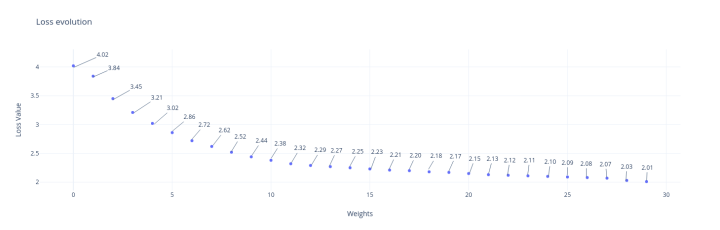
\includegraphics[width=\linewidth]{../images/loss_evolution.png}
  \caption{loss growth}
  \label{Figure 1}
\end{figure}
\section*{Results}
\subsection*{Metrics}
\begin{flushright}
  \begin{minipage}[t]{0.96\linewidth}\
    Due to the nature of music and creative composition according to Yang [12], it becomes necessary to identify methods of evaluation with which to compare the effectiveness of the LSTM and Markov generated music. In order to achieve a broad spectrum of analysis, multiple types of results were compiled to achieve tangible metrics:
    \begin{itemize}
        \item Frequency spectrum analysis compared to Beethoven compositions
        \item Heatmaps of note uage frequency in each model and their difference
        \item Opinion based survey
    \end{itemize}
  \end{minipage}
\end{flushright}
\subsection*{Frequency spectrum analysis}
\begin{flushright}
  \begin{minipage}[t]{0.96\linewidth}\
    In the section below, we will cover the frequency-domain analysis which will help us examine how the characteristic of the value of each component of a signal in frequency changes over time. Within the frequencies we are looking for an uniformly distributed graph. \\
  \end{minipage}
  \begin{figure}
    \centering
    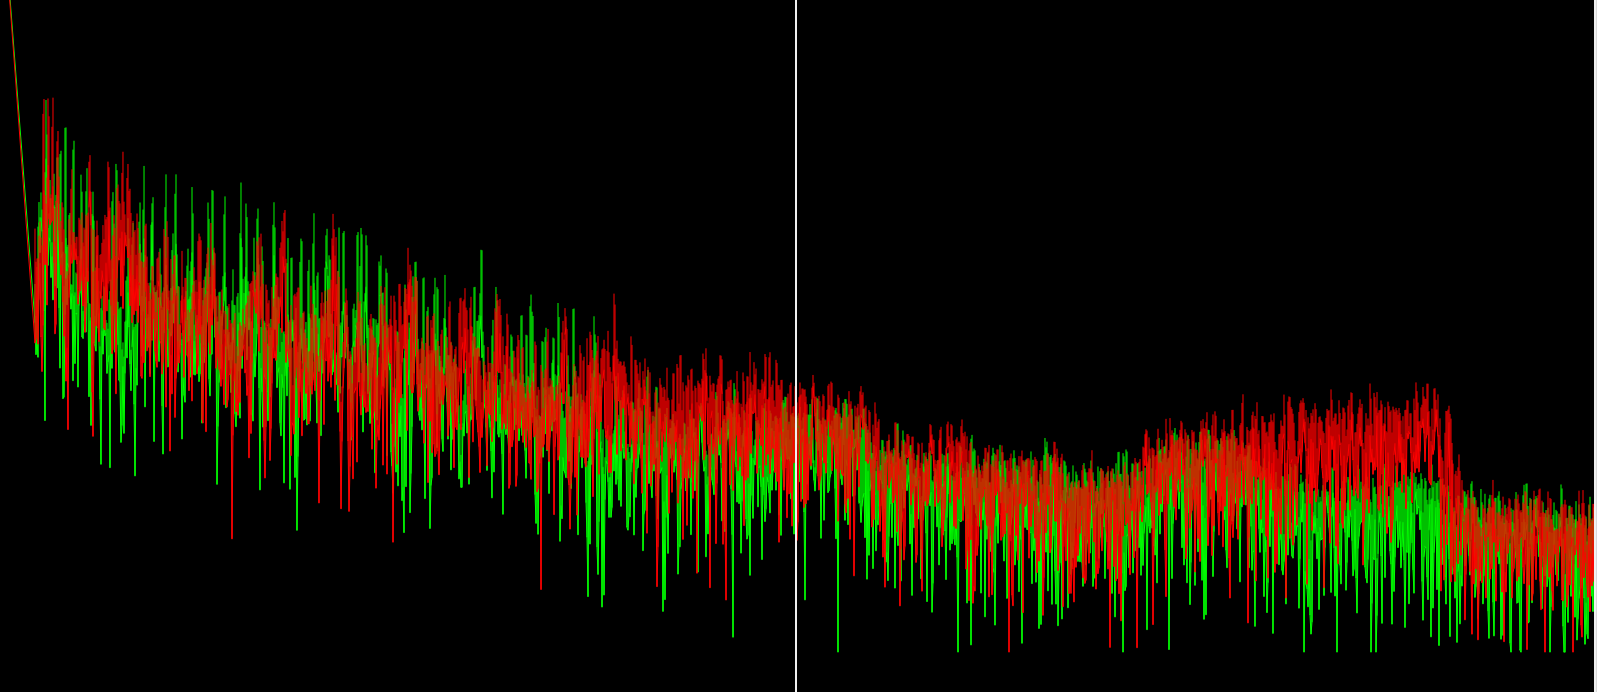
\includegraphics[scale=0.3]{../images/diff_LSTM_Beeth}
    \caption{Figure 2. Frequency spectrum between Beethoven song and LSTM generated midi}
    \label{Figure 2}
    \vspace{1cm}
    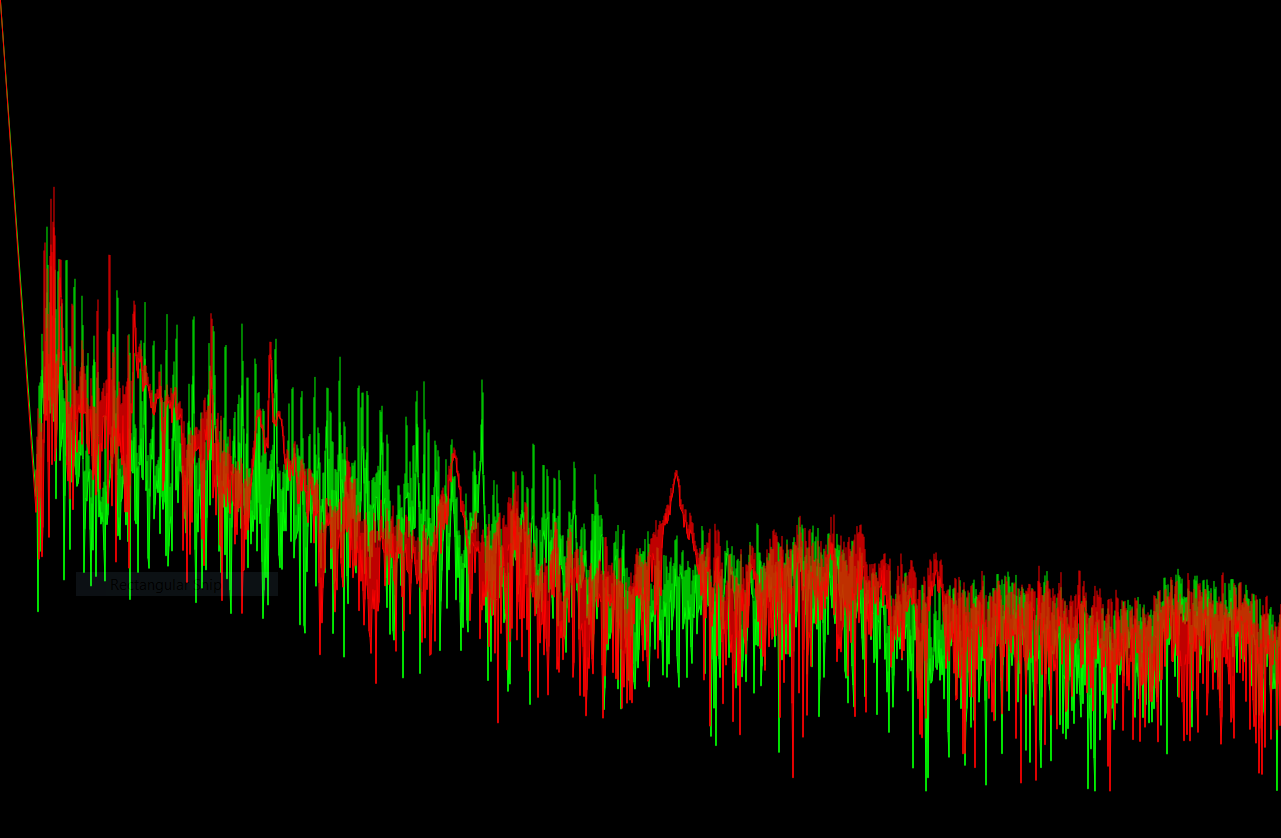
\includegraphics[scale=0.3]{../images/diff_HMM_Beeth}
    \caption{Figure 3. Frequency spectrum between Beethoven song and Hidden Markov Model song}
    \label{Figure 3}
  \end{figure}
\end{flushright}
\begin{flushright}
  \begin{minipage}[t]{0.96\linewidth}\
    Now we can compare how the frequency spectrum behaves in both the models compared to a Beethoven song. In both of the figures the red frequency represents the generated songs and green represents the Beethoven song. In figure 2, we notice constant fluctuations of the red frequency which clearly shows higher frequencies than the Beethoven song. In fact, the generated song is not uniformly distributed, it is dispersedly distributed leading to a more messy and scattered melody[4, para. 4.3]. This can be seen in the right side of the frequency spectrum where there is a big peak. In figure 3, the red frequency represents the Hidden Markov Model generated song. We can observe that the frequencies are more uniformly distributed and the high frequencies are lower than then LSTM which makes the melody less scattered and messy[4, para 4.3]. In the middle of the frequency spectrum, a peak of the graph is observed before returning back to a uniform distribution. This peak remains lower than the peak of figure 2, demonstrating higher cohesion in the song.
  \end{minipage}
\end{flushright}
\subsection*{Note occurrence frequency}
\begin{flushright}
  \begin{minipage}[t]{0.96\linewidth}\

  \end{minipage}
\end{flushright}
\subsection*{Survey}
\begin{flushright}
  \begin{minipage}[t]{0.96\linewidth}\

  \end{minipage}
\end{flushright}
\section*{Conclusions}
\begin{flushright}
  \begin{minipage}[t]{0.96\linewidth}\

  \end{minipage}
\end{flushright}
\section*{References}
\begin{flushright}
  \begin{minipage}[t]{0.96\linewidth}\

  \end{minipage}
\end{flushright}
\end{document}
